\section{Introduction}
\label{sec:introduction}

\subsection{Contexte}

Proposer un placement à un client est un exercice à trois volets. Il faut d'abord \emph{connaître le client} : son horizon, sa situation financière, sa capacité réelle à supporter une perte. Il faut ensuite \emph{lire le marché} : une même allocation n'a pas le même risque dans une période calme et au cœur d'une crise. Il faut enfin \emph{justifier} la recommandation, ce que la réglementation impose aux conseillers et ce que le client est en droit d'attendre.

L'apprentissage automatique semble bien armé pour chacun de ces volets : classer des clients à partir de leurs caractéristiques, repérer des états de marché, prévoir des rendements. La littérature appelle pourtant à la prudence. La prévision des rendements financiers est notoirement difficile : la plupart des variables proposées ne battent pas, hors échantillon, une simple moyenne historique~\cite{welch2008}, et les gains obtenus par l'apprentissage automatique restent modestes même avec des données très riches~\cite{gu2020}. De même, les portefeuilles optimisés battent rarement la règle naïve qui répartit le capital à parts égales~\cite{demiguel2009}. Enfin, les données financières se prêtent à des erreurs méthodologiques, les \emph{fuites de données}, qui produisent des performances spectaculaires sur le papier et décevantes en réalité~\cite{lopezdeprado2018}.

\subsection{Problématique et objectifs}

Notre problématique est la suivante : \emph{comment construire un assistant qui recommande à chaque client un portefeuille adapté à son profil et à l'état du marché, explique sa recommandation, et dont on puisse mesurer honnêtement la valeur ?}

Nous nous sommes fixé quatre objectifs :
\begin{enumerate}
  \item \textbf{Couvrir les familles de méthodes du cours}~\cite{cours_ml} sur un problème réel : apprentissage supervisé (classification et régression), non supervisé (clustering, détection d'anomalies), réduction de dimension, apprentissage par renforcement et interprétabilité.
  \item \textbf{Évaluer sans fuite de données}, avec des références simples (\emph{baselines}) et des tests statistiques, et accepter les conclusions négatives.
  \item \textbf{Rendre chaque décision explicable}, au niveau global (quelles variables comptent) et au niveau d'un client (pourquoi ce profil, pourquoi ce portefeuille).
  \item \textbf{Livrer un outil utilisable} : une application web que l'on peut essayer en ligne ou réinstaller à partir du dépôt.
\end{enumerate}

\subsection{Approche : un système multi-agent}

Plutôt qu'un modèle unique, nous avons découpé le problème en tâches confiées à des \emph{agents} spécialisés~\cite{wooldridge2009}. Chaque agent répond à une seule question avec la famille de méthodes la plus adaptée (tableau~\ref{tab:agents}). Les agents communiquent par un \emph{tableau noir} partagé, et un orchestrateur les appelle dans l'ordre, avec une boucle de négociation entre l'agent Allocation et l'agent Risque (figure~\ref{fig:architecture}).

\begin{table}[H]
  \centering
  \small
  \caption{Les sept agents, la question qu'ils traitent et les méthodes comparées.}
  \label{tab:agents}
  \begin{tabularx}{\textwidth}{@{}l L l L@{}}
    \toprule
    \textbf{Agent} & \textbf{Question traitée} & \textbf{Paradigme} & \textbf{Méthodes comparées} \\
    \midrule
    Profil      & Le client peut-il supporter des pertes ? & Classification & Logistique, KNN, SVM, arbre, forêt, boosting, MLP ; SMOTE, ADASYN \\
    Prévision   & Quels actifs surperformeront le mois prochain ? & Régression temporelle & MCO, Ridge, Lasso, Elastic Net, KNN, SVR, arbres, boosting, MLP ; ACP \\
    Régime      & Le marché est-il calme ou stressé ? & Clustering & K-means, CAH, DBSCAN, mélange gaussien \\
    Alerte      & La journée est-elle anormale ? & Anomalies & z-score, Grubbs, gaussienne, Isolation Forest, LOF, One-Class SVM \\
    Risque      & Quel est le risque du portefeuille ? & Statistique & Ledoit-Wolf, VaR, CVaR \\
    Allocation  & Quel portefeuille choisir ? & Optimisation, renforcement & Moyenne-variance (Black-Litterman), parité de risque, HRP, PPO \\
    Explication & Pourquoi cette recommandation ? & Interprétabilité & Coefficients, permutation, SHAP \\
    \bottomrule
  \end{tabularx}
\end{table}

\begin{figure}[H]
  \centering
  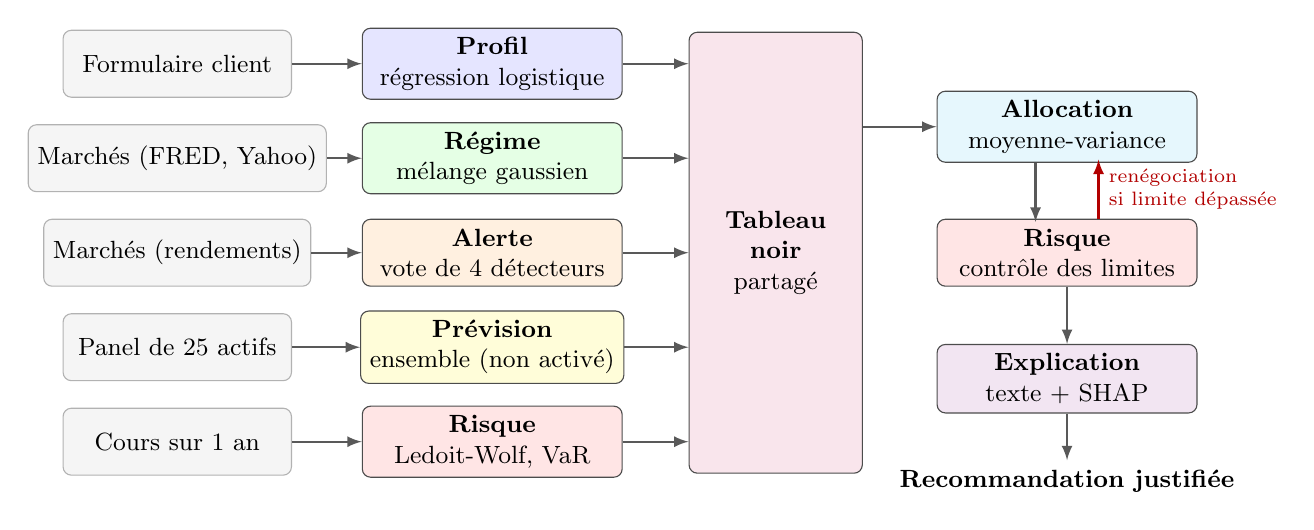
\begin{tikzpicture}[
      font=\small,
      src/.style={draw=gray!60, fill=gray!8, rounded corners=3pt, minimum width=2.9cm, minimum height=0.85cm, align=center},
      ag/.style={draw=black!70, rounded corners=3pt, minimum width=3.3cm, minimum height=0.85cm, align=center},
      fl/.style={-latex, thick, gray!70!black}]
    % Sources
    \node[src] (s1) at (0, 3.0) {Formulaire client};
    \node[src] (s2) at (0, 1.8) {Marchés (FRED, Yahoo)};
    \node[src] (s3) at (0, 0.6) {Marchés (rendements)};
    \node[src] (s4) at (0,-0.6) {Panel de 25 actifs};
    \node[src] (s5) at (0,-1.8) {Cours sur 1 an};
    % Agents d'analyse
    \node[ag, fill=blue!10]   (pr) at (4, 3.0) {\textbf{Profil}\\ régression logistique};
    \node[ag, fill=green!10]  (re) at (4, 1.8) {\textbf{Régime}\\ mélange gaussien};
    \node[ag, fill=orange!12] (al) at (4, 0.6) {\textbf{Alerte}\\ vote de 4 détecteurs};
    \node[ag, fill=yellow!15] (pv) at (4,-0.6) {\textbf{Prévision}\\ ensemble (non activé)};
    \node[ag, fill=red!10]    (ri) at (4,-1.8) {\textbf{Risque}\\ Ledoit-Wolf, VaR};
    % Tableau noir
    \node[ag, fill=purple!10, minimum height=5.6cm, minimum width=2.2cm] (bb) at (7.6, 0.6) {\textbf{Tableau}\\ \textbf{noir}\\ partagé};
    % Décision
    \node[ag, fill=cyan!10]   (alc) at (11.3, 2.2) {\textbf{Allocation}\\ moyenne-variance};
    \node[ag, fill=red!10]    (ctl) at (11.3, 0.6) {\textbf{Risque}\\ contrôle des limites};
    \node[ag, fill=violet!10] (ex)  at (11.3,-1.0) {\textbf{Explication}\\ texte + SHAP};
    \node[align=center, font=\small\bfseries] (out) at (11.3,-2.3) {Recommandation justifiée};
    \foreach \a/\b in {s1/pr, s2/re, s3/al, s4/pv, s5/ri} \draw[fl] (\a) -- (\b);
    \foreach \a in {pr, re, al, pv, ri} \draw[fl] (\a.east) -- (bb.west |- \a.east);
    \draw[fl] (bb.east |- alc.west) -- (alc.west);
    \draw[fl] (alc.south) ++(-0.4,0) -- ++(0,-0.75);
    \draw[fl, red!70!black] (ctl.north) ++(0.4,0) -- ++(0,0.75) node[midway, right, font=\scriptsize, align=left] {renégociation\\si limite dépassée};
    \draw[fl] (ctl) -- (ex);
    \draw[fl] (ex) -- (out);
  \end{tikzpicture}
  \caption{Architecture du système. Les agents d'analyse déposent leurs conclusions sur le tableau noir ; l'agent Allocation propose un portefeuille que l'agent Risque accepte ou renvoie avec une contrainte plus stricte ; l'agent Explication rédige la recommandation.}
  \label{fig:architecture}
\end{figure}

Ce découpage a trois avantages. Chaque agent peut être évalué \emph{séparément}, avec la métrique et la référence qui lui conviennent. Un agent qui n'apporte rien peut être \emph{désactivé} sans toucher aux autres : c'est ce qui arrive à l'agent Prévision (section~\ref{sec:prevision}). Enfin, la chaîne de décision est \emph{lisible} : le journal des échanges sur le tableau noir montre qui a décidé quoi.

\subsection{Démarche}

Nous avons suivi pour chaque agent le processus de développement présenté en cours : compréhension du problème, collecte et nettoyage des données, analyse exploratoire, préparation, séparation entraînement / validation / test, entraînement, évaluation, optimisation des hyperparamètres, puis déploiement. Une règle traverse tout le projet : \textbf{la période de test ne sert à aucun choix}. Tous les réglages (modèle retenu, seuils, hyperparamètres, paramètres de l'allocation) sont fixés sur la validation, et le test sert à une évaluation unique.

L'ensemble est reproductible : un notebook unique, organisé dans le même ordre que ce rapport, s'exécute de bout en bout en 22 minutes et produit tous les tableaux et figures cités. Le code, les données et les modèles sont publiés sur GitHub\footnote{\url{https://github.com/kissou-alain/Assistant-Portefeuille-financier}}, et l'application est accessible en ligne\footnote{\url{https://assistant-portefeuille-financier.vercel.app}}.

\subsection{Organisation du rapport}

La section~\ref{sec:donnees} présente les données et le protocole qui empêche les fuites. Les sections~\ref{sec:profil} à~\ref{sec:regime_alerte} détaillent les agents d'apprentissage : Profil (classification), Prévision (régression temporelle), Régime et Alerte (non supervisé). La section~\ref{sec:systeme} décrit leur assemblage, la section~\ref{sec:allocation_backtest} l'allocation et son évaluation historique, et la section~\ref{sec:renforcement} l'alternative par renforcement. La section~\ref{sec:application} présente l'application. Nous discutons enfin la pertinence de la démarche, sa valeur ajoutée et ses limites (section~\ref{sec:discussion}), avant de conclure sur les perspectives et sur ce que ce projet nous a appris (section~\ref{sec:conclusion}).
